% PDF 生成時のテンプレートファイル。SATySFi で生成した文書本体(main.tex)を読み込んでコンパイルする。
\documentclass[uplatex]{jsarticle}

% パッケージの読み込み
\usepackage{amsmath,amssymb}
\usepackage{framed,color}
\usepackage[dvipdfmx]{graphicx}
\usepackage{hyperref}
\usepackage{listings}
\usepackage{upquote}

% パッケージの設定
\lstset{
  basicstyle={\ttfamily},
  identifierstyle={\small},
  commentstyle={\smallitshape},
  keywordstyle={\small\bfseries},
  ndkeywordstyle={\small},
  stringstyle={\small\ttfamily},
  frame={tb},
  breaklines=true,
  columns=[l]{fullflexible},
  numbers=left,
  xrightmargin=0zw,
  xleftmargin=1.5zw,
  numberstyle={\scriptsize},
  stepnumber=1,
  numbersep=1zw,
  lineskip=-0.5ex,
  keepspaces=true,
  captionpos=b,
}

% コマンドの定義。SATySFi 文書中でのみ利用するコマンドは local.satyh-latex で定義する方が望ましいが、
% \title にも利用するため、ここで定義している。
\newcommand{\SATySFi}{SAT\kern-.2em\lower.5ex\hbox{Y}SF\kern-.0667em\lower.5ex\hbox{I}}

\title{\SATySFi\ \LaTeX\ Template}
\author{pickoba}

\begin{document}

\maketitle



このリポジトリは、\SATySFi で\LaTeX 文書を作成するテンプレートです。VS Code の Dev Container か Gitpod での使用を想定しています。

\section{文書のコンパイル}

VS Code 上で \verb$main.saty$ を開いている場合、以下のいずれかの方法で文書をコンパイルすることができます。

\begin{enumerate}
  \item ショートカットキー \verb$ctrl$/\verb$cmd$ + \verb$alt$ + \verb$b$
  \item エディタ右上のボタン(再生マーク)
\end{enumerate}


統合ターミナルで \verb$make document.pdf$ を実行することでもコンパイルできます。

\section{利用可能なコマンド}

\LaTeX のコマンドをラップする各種コマンドが \verb$latex-base.satyh-latex$ 内に定義されています。

\subsection{段落・節}

通常の段落は \verb$+p$ で、インデントなしの段落は \verb$+pn$ で作成できます。引数は段落の内容を示すインラインテキストです。

\begin{lstlisting}
+p{
  normal paragraph
}
+pn{
  no indent paragraph
}
\end{lstlisting}

節は \verb$+section$ と \verb$+subsection$ で作成できます。第一引数は節のタイトルを示すインラインテキスト、第二引数は節の内容を示すブロックテキストです。

\begin{lstlisting}
+section{ section title }<
  +p{
    section content
  }
  +subsection{ subsection title }<
    +p{
      subsection content
    }
  >
>
\end{lstlisting}

\subsection{テキスト装飾}

\verb$\textbf$, \verb$\textit$ が利用可能です。

\begin{lstlisting}
+p{
  \textbf{bold string}, \textit{italic string}
}
\end{lstlisting}

\begin{oframed}
  
  \textbf{bold string}, \textit{italic string}
\end{oframed}

\subsection{箇条書き}

番号付き箇条書きは \verb$+enumerate$ で、番号なし箇条書きは \verb$+itemize$ で作成できます。箇条書きの各要素は \verb$*$ で開始し、その数を増やすことで入れ子構造を作成できます。

\begin{lstlisting}
+enumerate{
  * item 1
  * item 2
    ** item 2-1
    ** item 2-2
  * item 3
}
\end{lstlisting}

\begin{oframed}
  
  
  \begin{enumerate}
    \item item 1
    \item item 2
    \begin{enumerate}
      \item item 2-1
      \item item 2-2
    \end{enumerate}
    \item item 3
  \end{enumerate}
\end{oframed}

段落の途中で箇条書きを挿入したい場合は、インラインコマンド版の \verb$\enumerate$ と \verb$\itemize$ を利用できます。

\begin{lstlisting}
+p{
  paragraph text
  \itemize{
    * item 1
    * item 2
  }
  paragraph text
}
\end{lstlisting}

\begin{oframed}
  
  paragraph text
  
  \begin{itemize}
    \item item 1
    \item item 2
  \end{itemize}
  
  paragraph text
\end{oframed}

\subsection{コードブロック}

コードブロックは \verb$+code$ で作成できます。引数はコードの内容を示す文字列です。

\begin{lstlisting}
+code(```
#include <stdio.h>

int main() {
  printf("Hello, world!\n");
  return 0;
}
```);
\end{lstlisting}

\begin{oframed}
  
  \begin{lstlisting}
#include <stdio.h>

int main() {
  printf("Hello, world!\n");
  return 0;
}
  \end{lstlisting}
\end{oframed}

\subsection{画像の挿入}

画像は \verb$+figure$, \verb$\figure$ で挿入できます。引数は \verb$figure$ 型の値で、通常 \verb$include-graphics$ 関数を利用して作成します。配置はオプション引数で指定できます。

\verb$include-graphics$ 関数は画像ファイルのパスを必須引数に取り、オプション引数として中央寄せをするかどうかを示す \verb$centering$ と画像サイズを示す \verb$scale$ を指定できます。

\begin{lstlisting}
+figure(include-graphics ?(centering = true, scale = 0.2) `images/sunset.jpg`);
\end{lstlisting}



\begin{figure}[h]
  \centering
  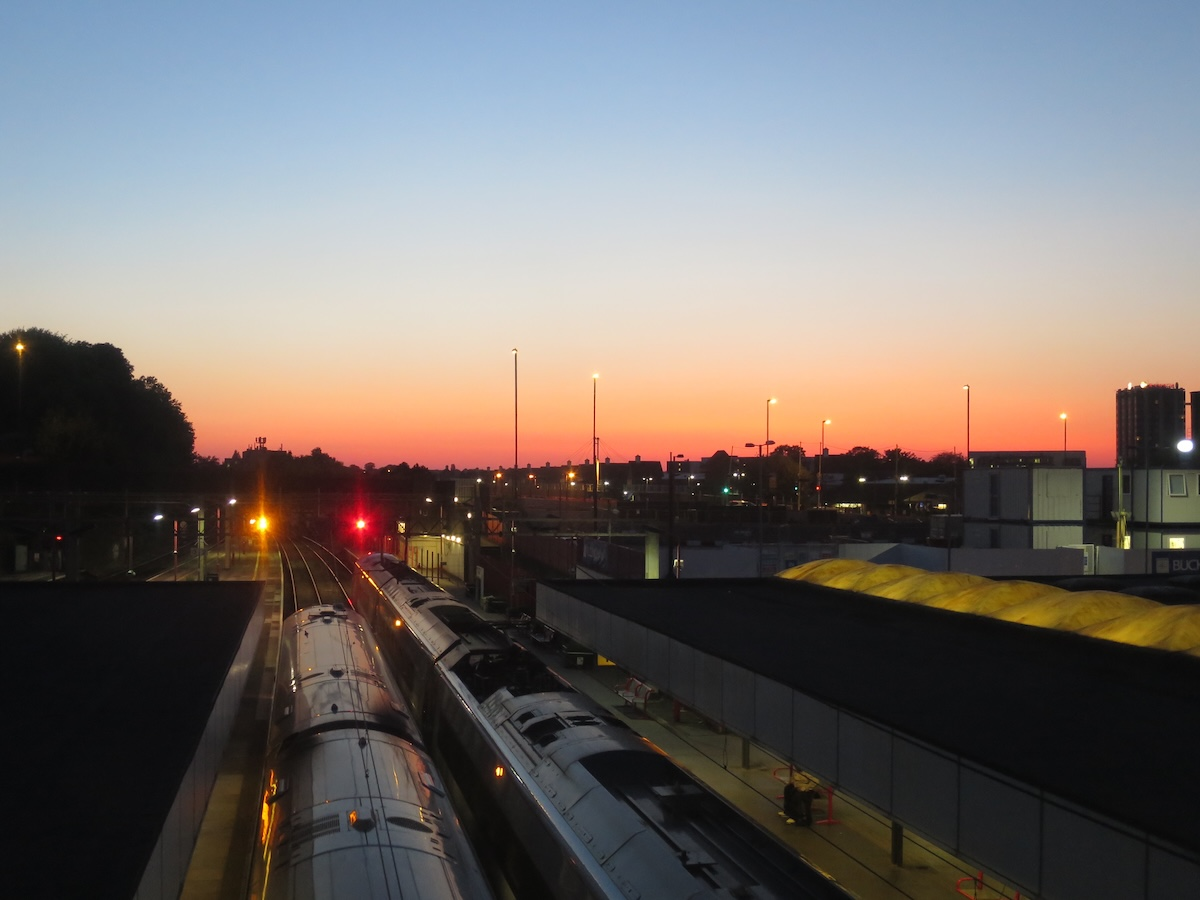
\includegraphics[keepaspectratio,scale=0.2]{images/sunset.jpg}
\end{figure}

画像にキャプションをつけたい場合、\verb$with-caption$ 関数を利用します。オプション引数としてラベルを指定でき、\verb$\ref$ で参照できます。\verb$with-caption \{caption\} (include-graphics ...)$ と書いても良いですが、パイプライン演算子 \verb$|>$ を利用して \verb$include-graphics ... |> with-caption \{caption\}$ と書くこともできます。

\begin{lstlisting}
+figure(
  include-graphics ?(centering = true, scale = 0.3) `images/sunset.jpg`
  |> with-caption ?(label = `fig:editor`) {Sunset}
);
+p{
  See figure \ref(`fig:editor`);.
}
\end{lstlisting}



\begin{figure}[h]
  \centering
  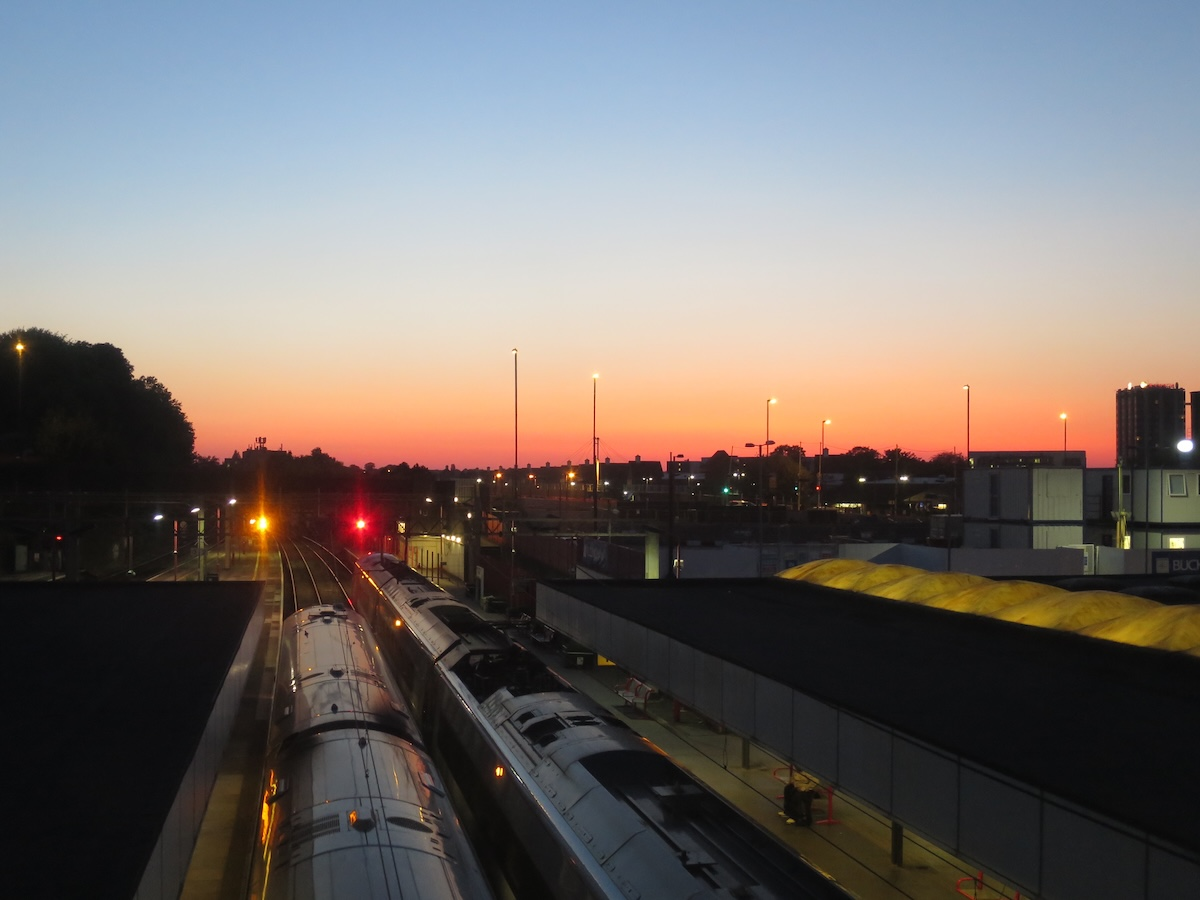
\includegraphics[keepaspectratio,scale=0.3]{images/sunset.jpg}
  \caption{Sunset}
  \label{fig:editor}
\end{figure}

\begin{oframed}
  
  See figure \ref{fig:editor}.
\end{oframed}

\section{連絡先}

バグ報告等あれば以下にご連絡ください。

\begin{itemize}
  \item GitHub (Template): \href{https://github.com/pickoba/satysfi-latex-template}{pickoba/satysfi-latex-template}
  \item \SATySFi  Slack: @pickoba
\end{itemize}


\end{document}
